\begin{frame}{RIVET}
\begin{itemize}
\item<1-> Let's think about how this could go wrong and how we could fix it!
\item<2-> Suppse that, instead of data that look like this:
\begin{figure}
\begin{tikzpicture}[scale = 1.5]
    \draw plot[mark=*, mark size = 0.5, only marks] file {data/data3.txt};
\end{tikzpicture}
\end{figure} 
\end{itemize}
\end{frame}
%---------------------------------------------------------------
\begin{frame}{RIVET}
\begin{itemize}
\item Let's think about how this could go wrong and how we could fix it!
\item We instead had data that looked like this:
\begin{figure}
\begin{tikzpicture}[scale = 1.5]
    \draw plot[mark=*, mark size = 0.5, only marks] file {data/data3.txt};
    \draw[fill=black] (-0.3,-0.4) circle (.5pt);
    \draw[fill=black] (-0.25,0.5) circle (.5pt);
    \draw[fill=black] (-0.5,0.1) circle (.5pt);
    \draw[fill=black] (0,0) circle (.5pt);
    \draw[fill=black] (0.1,-0.5) circle (.5pt);
    \draw[fill=black] (0.5,-0.3) circle (.5pt);
    \draw[fill=black] (0.2,0.4) circle (.5pt);
    \draw[fill=black] (0.4,0.1) circle (.5pt);
\end{tikzpicture}
\end{figure} 
\end{itemize}
\end{frame}
%---------------------------------------------------------------
\begin{frame}{RIVET}
These red points look like noise.
\begin{figure}
\begin{tikzpicture}[scale = 1.5]
    \draw plot[mark=*, mark size = 0.5, only marks] file {data/data3.txt};
    \draw[red, fill=red] (-0.3,-0.4) circle (.5pt);
    \draw[red, fill=red] (-0.25,0.5) circle (.5pt);
    \draw[red, fill=red] (-0.5,0.1) circle (.5pt);
    \draw[red, fill=red] (0,0) circle (.5pt);
    \draw[red, fill=red] (0.1,-0.5) circle (.5pt);
    \draw[red, fill=red] (0.5,-0.3) circle (.5pt);
    \draw[red, fill=red] (0.2,0.4) circle (.5pt);
    \draw[red, fill=red] (0.4,0.1) circle (.5pt);
\end{tikzpicture}
\end{figure} 
\end{frame}
%---------------------------------------------------------------
\begin{frame}{RIVET}
The first barcode does not have the red point 'noise'.  The second barcode includes the red point 'noise'.

\begin{figure}
\centering
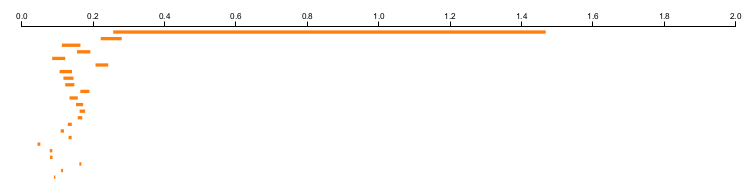
\includegraphics[scale=0.5]{images/data3rip.png}
\end{figure} 

\begin{figure}
\centering
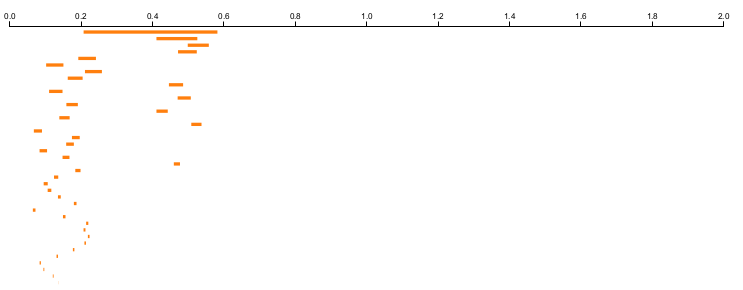
\includegraphics[scale=0.5]{images/data7rip.png}
\end{figure} 
\end{frame}
%---------------------------------------------------------------
\begin{frame}{RIVET}
\begin{itemize}
\item<1-> One way to deal with such situations: consider the density of the points.
\item<2-> The red points are much less dense than the black points.
\item<3-> Set a density threshold -- only include points that satisfy that threshold.
\item<4-> Letting the density threshold vary results in \textit{multiparameter persistence}!
\end{itemize}
\begin{figure}
\begin{tikzpicture}[scale = 1.5]
    \draw plot[mark=*, mark size = 0.5, only marks] file {data/data3.txt};
    \draw[red, fill=red] (-0.3,-0.4) circle (.5pt);
    \draw[red, fill=red] (-0.25,0.5) circle (.5pt);
    \draw[red, fill=red] (-0.5,0.1) circle (.5pt);
    \draw[red, fill=red] (0,0) circle (.5pt);
    \draw[red, fill=red] (0.1,-0.5) circle (.5pt);
    \draw[red, fill=red] (0.5,-0.3) circle (.5pt);
    \draw[red, fill=red] (0.2,0.4) circle (.5pt);
    \draw[red, fill=red] (0.4,0.1) circle (.5pt);
\end{tikzpicture}
\end{figure} 
\end{frame}
%---------------------------------------------------------------
\begin{frame}{RIVET}
\begin{itemize}
\item<1-> Michael Lesnick and Matthew Wright have written a program for visualizing multiparameter persistence.\cite{lesnick2015interactive}
\item<2-> Installation is not so simple -- let us go through it together!
\end{itemize}
\end{frame}